%; whizzy section -pdf xpdf -latex ./whizzypdfptex.sh
% latex beamer presentation.
% platex, latex-beamer でコンパイルすることを想定。 

%     Tokyo Debian Meeting resources
%     Copyright (C) 2008 Junichi Uekawa

%     This program is free software; you can redistribute it and/or modify
%     it under the terms of the GNU General Public License as published by
%     the Free Software Foundation; either version 2 of the License, or
%     (at your option) any later version.

%     This program is distributed in the hope that it will be useful,
%     but WITHOUT ANY WARRANTY; without even the implied warranty of
%     MERCHANTABILITY or FITNESS FOR A PARTICULAR PURPOSE.  See the
%     GNU General Public License for more details.

%     You should have received a copy of the GNU General Public License
%     along with this program; if not, write to the Free Software
%     Foundation, Inc., 51 Franklin St, Fifth Floor, Boston, MA  02110-1301 USA

\documentclass[cjk,dvipdfmx,12pt]{beamer}
\usetheme{Tokyo}
\usepackage{monthlypresentation}

%  preview (shell-command (concat "evince " (replace-regexp-in-string "tex$" "pdf"(buffer-file-name)) "&"))
%  presentation (shell-command (concat "xpdf -fullscreen " (replace-regexp-in-string "tex$" "pdf"(buffer-file-name)) "&"))

%http://www.naney.org/diki/dk/hyperref.html
%日本語EUC系環境の時
\AtBeginDvi{\special{pdf:tounicode EUC-UCS2}}
%シフトJIS系環境の時
%\AtBeginDvi{\special{pdf:tounicode 90ms-RKSJ-UCS2}}

\title{東京エリア Debian 勉強会}
\subtitle{資料}
\author{岩松 信洋 iwamatsu@debian.or.jp\\IRC nick: iwamatsu}
\date{2008年6月21日}
\logo{
\includegraphics[width=8cm]{image200607/openlogo-light.eps}}

\begin{document}

\frame{\titlepage{}}


\section{Intro}

\emtext{設営準備にご協力ください}

\begin{frame}
 \frametitle{Agenda}
\begin{minipage}[t]{0.45\hsize}
  \begin{itemize}
  \item 注意事項
	\begin{itemize}
	 \item 飲食禁止
	 \item 政治/宗教/営利活動禁止
	\end{itemize}
  \item quiz
  \item 最近のDebian関連のイベント
	\begin{itemize}
	 \item 前回 
	\end{itemize}
 \end{itemize}
\end{minipage} 
\begin{minipage}[t]{0.45\hsize}
 \begin{itemize}
  \item dpatch/debhelperで作成するパッケージ作成方法
  \item Debian GNU/Hurd について熱く語る会
  \item 月刊 kFreeBSD / Nexenta / Hurd / SuperH
 \end{itemize}
\end{minipage}
\end{frame}

\section{最近}


\begin{frame}
 \frametitle{前回のAgenda}
\begin{minipage}[t]{0.45\hsize}
  \begin{itemize}
  \item 注意事項
	\begin{itemize}
	 \item 飲食禁止
	 \item 政治/宗教/営利活動禁止
	\end{itemize}
  \item quiz
  \item 最近のDebian関連のイベント
	\begin{itemize}
	 \item 前回 
	\end{itemize}
 \end{itemize}
\end{minipage} 
\begin{minipage}[t]{0.45\hsize}
 \begin{itemize}
  \item eeePC Open Source Developer's Conference
  \item 複数のバイナリパッケージを生成するソースパッケージの作成
  \item OpenSSL セキュリティーホール速報
  \item Debian 各種ポートアップデート(kFreeBSD, nexenta, Hurd, SuperH)
 \end{itemize}
\end{minipage}
\end{frame}


\section{DWN quiz}
\begin{frame}{Debian 常識クイズ}

Debian の常識、もちろん知ってますよね?
知らないなんて恥ずかしくて、知らないとは言えないあんなことやこんなこと、
みんなで確認してみましょう。

今回の出題範囲は\url{debian-devel-announce@lists.debian.org} に投稿された
内容とDebian Project Newsからです。

\end{frame}

\subsection{問題}

%問題をコピペ

 \santaku
 {Debian.ch(スイス連邦のDebianユーザグループ)の体制が変わりました。どうなったでしょう。}
 {前会計が辞任したので、Martin F. Krafft が会計になりました。}
 {会計を全てスイス銀行の管理下に置かれます。}
 {スイス連邦のPascal Couchepin大統領がDebianユーザになりました。}
 {A}

 \santaku
 {2008年6月5日に新しい Debian Policy がリリースされました。バージョン番号はいくつでしょうか。}
 {3.1415}
 {3.8.0.0}
 {4.0.0.0}
 {B}
 
 \santaku
 {Debian installer lenny beta 2がリリースされたのはいつでしょうか。}
 {実は上川さんの誕生日、5月22日}
 {2008年6月1日}
 {2008年6月10日}
 {C}

 \santaku
 {Perl の新しいバージョンの移行が完了しました。lennyに入る Perl のバージョンは? }
 {5.10}
 {5.20}
 {Perl-next-1.0}
 {A}

 \santaku
 {DPL から Bits from the DPL が出ました。あれ?今のDPLって?}
 {Sam Hocevar}
 {Martin Michlmayr}
 {Steve McIntyre}
 {C}

 \santaku
 {OpenSSHの DSA-1571 で影響を受けたパッケージ数はいくつでしょうか。}
 {20}
 {200}
 {2000}
 {A}

 \santaku
 {Debian Game team がデータの大きいサイズのパッケージについて提案したことは?}
 {データはP2Pで配信しようぜ!}
 {データはデータでアーカイブを分けようぜ!}
 {データは与えられるものではなく、与えるものだ!削除しましょう。}
 {B}

 \santaku
 {ftp-master teamが編成されました。FTP MasterはJoerg Jaspertと誰になったでしょう?}
 {Ryan Murray}
 {Junichi Uekawa}
 {Kenshi Muto}
 {A}

 \santaku
 {debconf の翻訳が完了一番乗りした国は?}
 {フランス}
 {日本}
 {実は翻訳状況の表示不具合で、まだ一番乗りはいません}
 {A}

 \santaku
 {debconf の翻訳が遅れていて、CFH を出した国は?}
 {ドイツ}
 {日本}
 {実は翻訳状況の表示ミスで、遅れていませんでした}
 {A}

 \santaku
 {Bastian Venthur と Noel Koetheレポートを出したイベントは?}
 {BSDCan 2008}
 {LinuxWorld Expo/Tokyo 2008}
 {LinuxTag 2008}
 {C}

\section{事前課題紹介}
\emtext{事前課題の紹介}
% pre work home work

\begin{frame}{事前課題問題}

\begin{enumerate}
 \item 「debhelper に追加してほしい機能/あったらいい機能」
 \item 「 Debian を使っていて他の distro にあるこの機能/パッケージがあれば…と思ったこと」
\end{enumerate}

\end{frame}

% (query-replace "\\subsection" "\\end{frame}\\begin{frame}")
% (query-replace "\\subsubsection" "\\textbf")

\begin{frame}{吉田@板橋}

お題:Debian を使っていて他の distro にあるこの機能/パッケージがあれば…
と思ったこと

1.ドライバーディスク機能

redhat系ディストリービューションにあるドライバーディスク機能は欲しいです
ね。特にDISK関連のドライバは無いとお手上げなので。
たびたび武藤さんの手(スペシャルカーネル入りiso作成)を煩わせないためには、
あるといいかなと思います。
#どっちみちドライバディスク作成で手が煩わされるかな(笑)
インストール後は、あまり吊し(Debian純正)のカーネルを使わないので困らない
のですが。次善はlenny等を入れて強制ダウングレードするのが手かな。

2.Xの自動起動停止

runlevelで制御したいとまでは言いませんが...
基本はXなしで速く、マウスなしでログイン
必要ならXを上げるというサーバっぽい運用が行いにくいです。


\end{frame}\begin{frame}{前田 耕平}

「Debian を使っていて他の distro にあるこの機能/パッケージがあれば…と
思ったこと」

Linuxじゃなくて、AIXなら楽だなぁと思う機能はあります。

\begin{itemize}
 \item LVM&ファイルシステムの拡張がAIXくらい楽にできれば良いなぁと思うことしばしば。
 \item システムバックアップの取得方法。mksysbコマンドのように楽に取れれば良いですね。
 \item エラーログの機能。errptコマンドでエラー情報を整形して表示できるのも良いです。
\end{itemize}

スキルレベルを標準化して運用要員を揃えるのなら、AIXは良いですね。自宅
では使いたくないですけど。w


\end{frame}\begin{frame}{あけど}

「 Debian を使っていて他の distro にあるこの機能/パッケージがあれば…と
思ったこと」

ずばり、「Hinemos」です。http://www.hinemos.info/
Redhat で動いてるくらいだからDebianで動かすのは難しくなさそうですが、aptに慣れてしまうとdebパッケージであれば…と思ってしまいます。

\end{frame}\begin{frame}{山本 浩之}

「Debian を使っていて他の distro にあるこの機能/パッケージがあれば…と
思ったこと」

TOMOYO Linux も公式に入ったことですし、AppArmor も早く公式に入って、セ
キュリティ・パッケージを強化すると嬉しい人が多そう。

\end{frame}\begin{frame}{藤沢 理聡}


「Debian を使っていて他の distro にあるこの機能/パッケージがあれば…と思っ 
たこと」

これまでサーバにしか使ってこなかったので、機能面の不足はあんまり感じたこと 
ありません。
機能ではありませんが、不足を最も感じていたのは認識してもらえないハードが 
RedHat系より
多いんじゃないか、ということです。実際のところはどうかわかりません 
が、「RedHatでは
認識したんだけど……」と思うことは少なからずありました。とはいっても、2年以上 
前の
ことなので、既に改善されているのかもしれませんが。

\end{frame}\begin{frame}{小林 儀匡}

「debhelper に追加してほしい機能/あったらいい機能」

Bug\#45614として提案されているdh\_{}alternativesが欲しいです。
alternativesを使用するパッケージを作成する場合、
ほとんどテンプレート化されているpostinstとprermと自分で書く必要がありますが、
メンテナスクリプトは極力メンテナに書かせないほうがよい気がするので……。


\end{frame}\begin{frame}{日比野 啓}

「debhelper に追加してほしい機能/あったらいい機能」

perl module のパッケージを作ることが多いので、
perl のプログラムでも、バイナリにおける dh\_{}shlibdeps みたいに
ライブラリの依存関係の検知を支援してくれるような機能が欲しいです。

Debian を使っていて他の distro にあるこの機能/パッケージがあれば…と思ったこと

Debianというよりはlinuxの話かもしれませんが、
AIXのerrptのような厳密なチェック機能はすばらしいと思います。
あとは、FreeBSDのktraceがちょっとうらやましいと思ったことがあります。
だいぶ昔のなのでうろおぼえなんですが、kernelの中までtraceしてくれたような。

\end{frame}\begin{frame}{岩松 信洋}

「Debian を使っていて他の distro にあるこの機能/パッケージがあれば…と思ったこと」

rpm にはドキュメントはインストールしないというオプションがあるのですが、Debian にはないので
インストール時に選択できるようにしてほしいです。
あと、他のディストリにはサポートしているのに Debian がサポート対象になっていないソフトウェアとか
けっこうあって(サイボウズさんとか)、それだけでDebianが使えないというのが悲しいです。


\end{frame}

% (query-replace "\\subsection" "\\end{frame}\\begin{frame}")
% (query-replace "\\subsubsection" "\\textbf")


\emtext{2008年計画}

\begin{frame}{2008年計画}

{\scriptsize
\begin{enumerate}
 \item 新年会「気合を入れる」
 \item Open Source Conference Tokyo (3/1)
 \item データだけのパッケージを作成してみる、
       ライセンスの考え方 (David Smith)
 \item バイナリ一つのパッケージを作成してみる (吉田@板橋)\\
       バージョン管理ツールを使いDebianパッケージを管理する(git)\\
       アップストリームの扱い(svn/git/cvs)(岩松 信洋さん)
 \item バイナリの分けたパッケージの作成。(前田さん)\\
       バイナリの分け方の考え方、アップグレードなどの運用とか。
 \item パッケージ作成(dpatch/debhelperで作成するパッケージ)(小林儀匡さん)\\
       man の書き方(roff or docbook)(でんさん)\\
       Open Source Conference Hokkaido
 \item パッケージ作成(kernel patch、kernel module)
       、Debconf発表練習
 \item Debconf アルゼンチン、共有ライブラリパッケージ作成

 \item Open Source Conference Tokyo/Fall、
       デーモン系のパッケージの作成、latex、 emacs-lisp、フォントパッケージ
 \item パッケージの cross-compile の方法、amd64 上で i386 のパッケージと
       か、OSC-Fall報告会、Debconf報告会
 \item 国際化 po-debconf / po化 / DDTP
 \item 忘年会
\end{enumerate}
}
\end{frame}

\emtext{dpatch/debhelperで作成するパッケージ作成方法}
\emtext{みんなも Debian GNU/Hurd を使おうよ!}
\emtext{月刊 kFreeBSD / Nexenta / Hurd / SuperH /eeepc}

\begin{frame}{宴会場所}
\begin{center}
 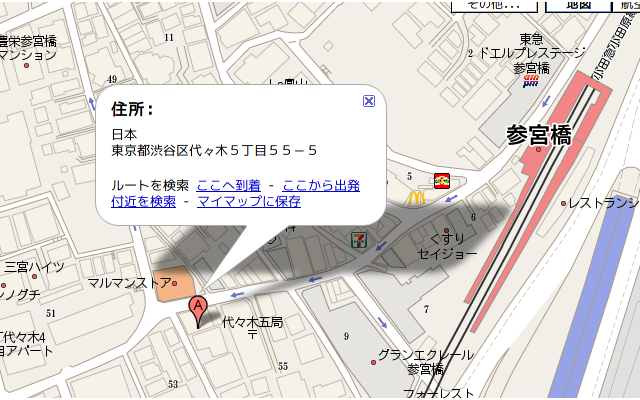
\includegraphics[width=0.7\hsize]{image200806/satsuki.png}
\end{center}

\begin{itemize}
 \item 宴会場所\\
       本日の宴会は「さつき」です。\\
       参加者はフロアに集合し、全員で移動しましょう。
 \item 片付け\\
       部屋を片付けるのにご協力ください。
\end{itemize}

\end{frame}

\end{document}

;;; Local Variables: ***
;;; outline-regexp: "\\([ 	]*\\\\\\(documentstyle\\|documentclass\\|emtext\\|section\\|begin{frame}\\)\\*?[ 	]*[[{]\\|[]+\\)" ***
;;; End: ***
